\documentclass[12pt]{article}
\usepackage{../../lecture_notes}
\usepackage{../../math}
\usepackage{../../uark_colors}

\hypersetup{
  colorlinks = true,
  allcolors = ozark_mountains,
  breaklinks = true,
  bookmarksopen = true
}

\begin{document}
\begin{center}
  {\Huge\bf RStudio Setup}
  
  \smallskip
  {\large\it  ECON 4753 — University of Arkansas}

  \medskip
  {\large Prof. Kyle Butts}
\end{center}

\section*{Opening RStudio}

When you open up RStudio, you will see 3 panels like in Figure \ref{fig:rstudio}. Let's walk through them. 
\begin{enumerate}
  \item First, we have the \textbf{Console} tab on the left-hand side. This area is where you will run R commands and text output will be displayed. For instance, try typing \texttt{1 + 1} and hit enter into the console. It should display \texttt{[1] 2}.
  
  \item Second, in the top-right you have the panel containing the \textbf{Environment} tab. This will show you information of all \textbf{variables} you make in your active R session. 
  
  \item Third, is a panel containing the \textbf{Files}, \textbf{Plots}, \textbf{Help}, \textbf{Viewer} tabs. The \textbf{Files} tab displays the filesystem which we will discuss below. \textbf{Plots} will be where figures you create will be shown (try typing \texttt{plot(mtcars\$hp, mtcars\$mpg)}). \textbf{Help} will display help information when you call it (try typing \texttt{?plot}). The \textbf{Viewer} tab will be where we can preview our Rmarkdown file.
\end{enumerate}



\begin{figure}[!ht]
  \caption{RStudio Window}
  \label{fig:rstudio}
  \centering
  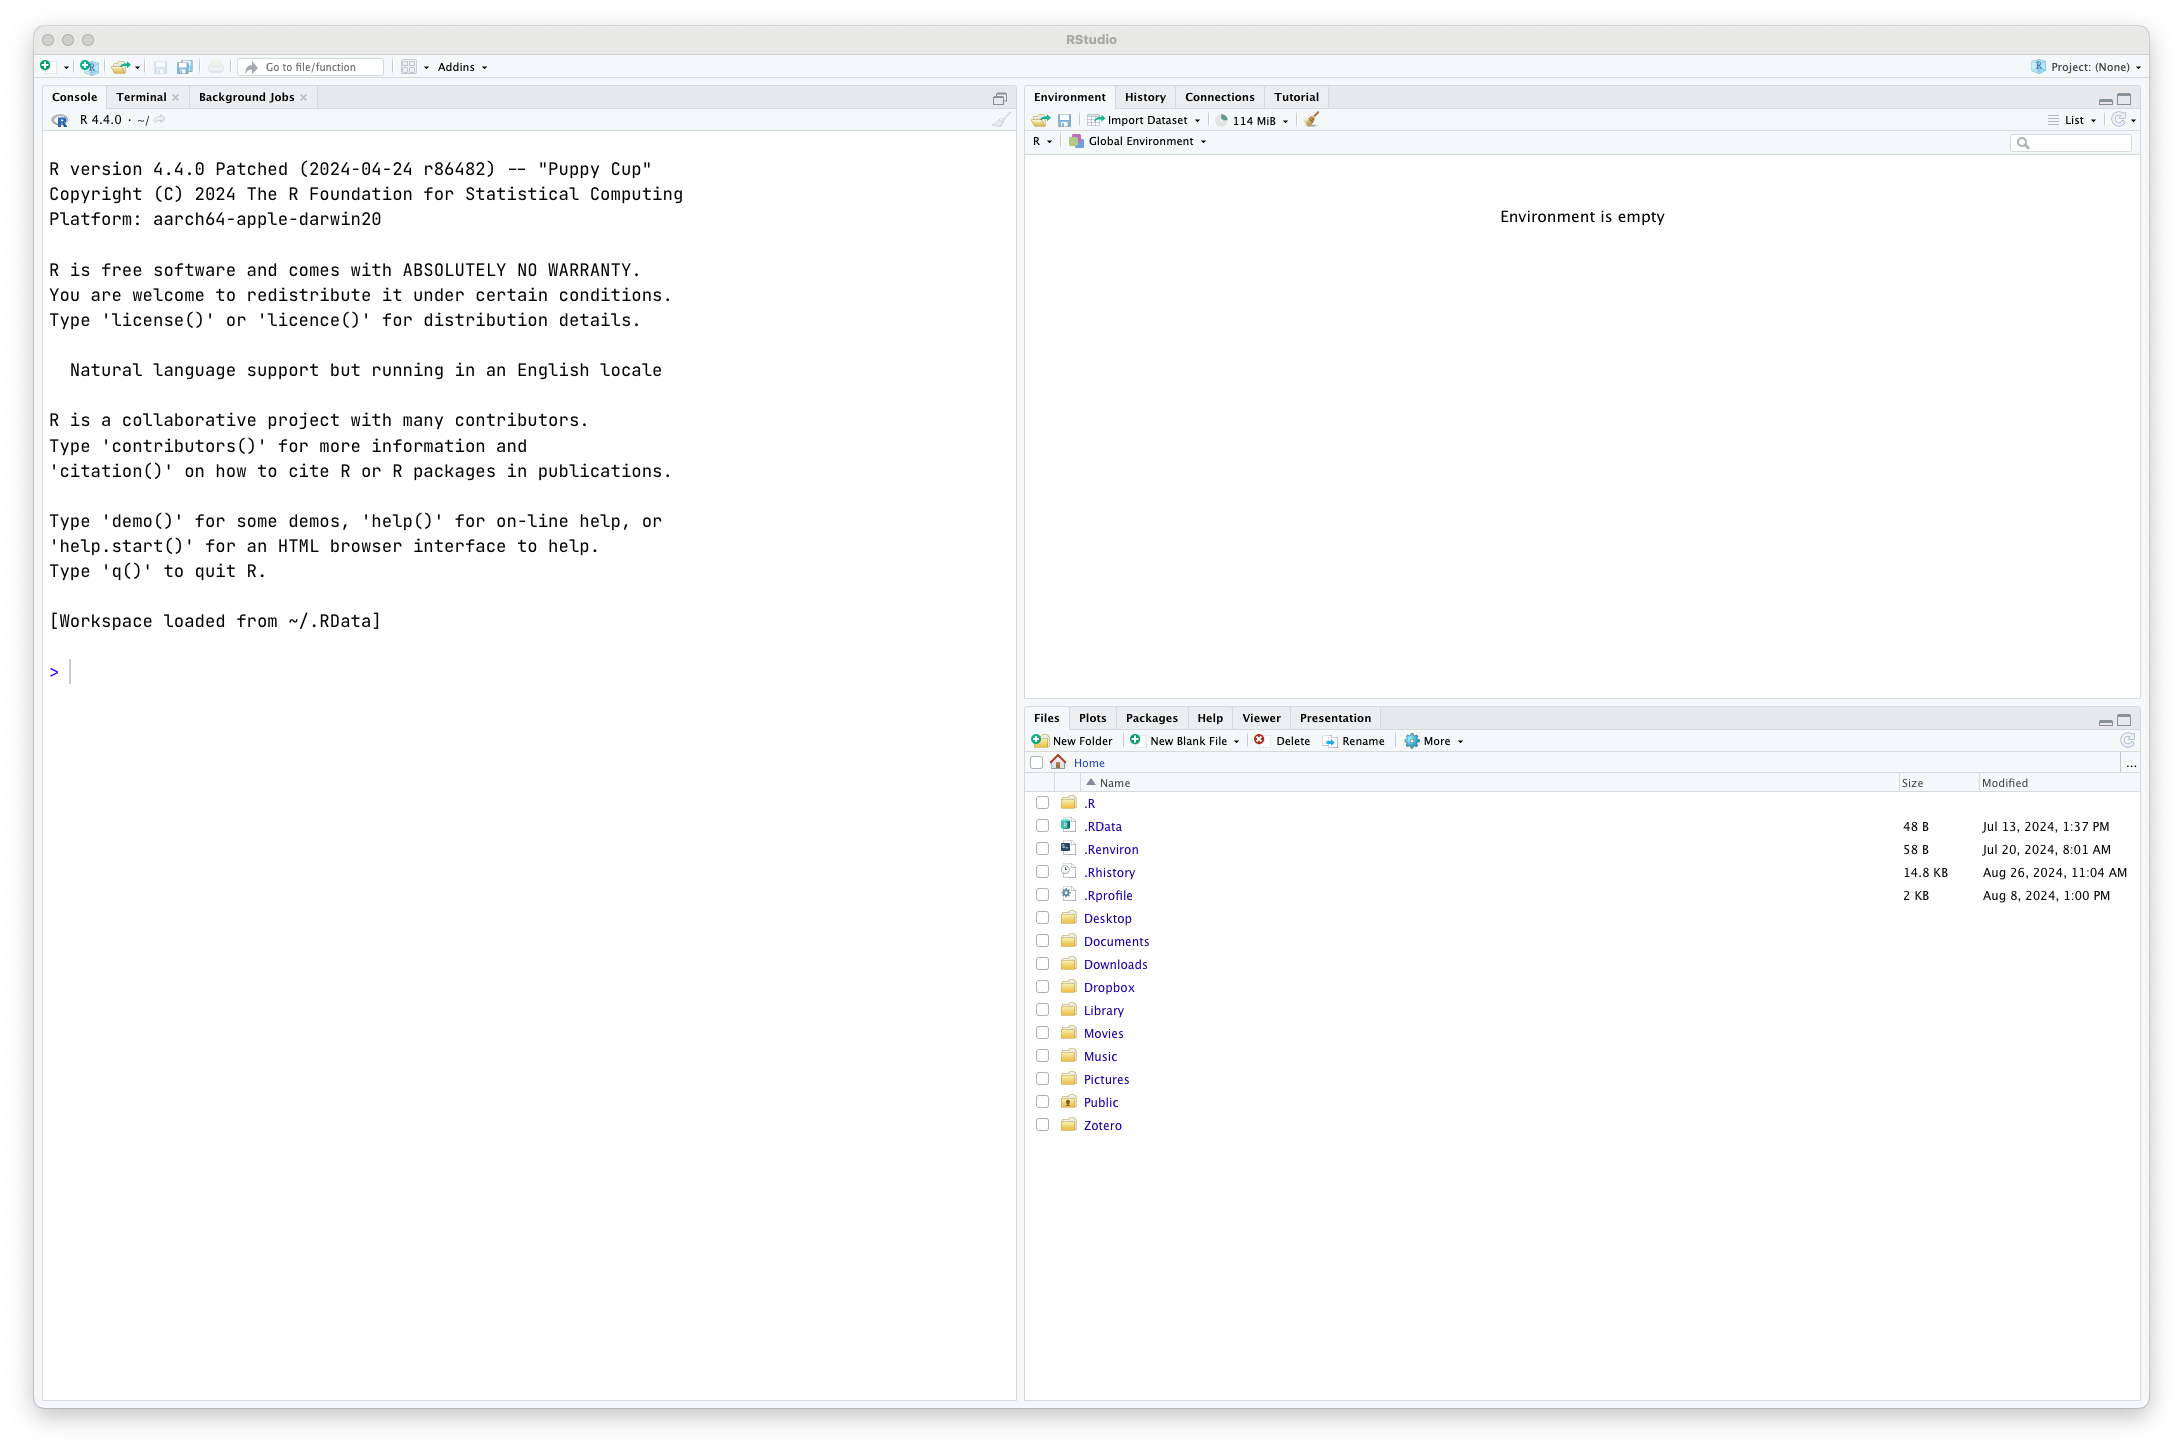
\includegraphics[width = 0.8\textwidth]{figures/rstudio.png}
\end{figure}


\subsection*{Files and Folders on your Computer}

If you are not familiar with the file system, here is a brief introduction in this and the following paragraph.\footnote{You can watch this three part tutorial if you're very new to computers: \url{https://www.youtube.com/watch?v=k-EID5_2D9U}.} It is important to understand how computers organize and store data. A computer's file system is essentially a large hierarchical structure that allows you to store and retrieve files and folders in an organized manner. At the top of this hierarchy is the root directory, which can be thought of as the main folder that contains everything else on your computer.

Within this root directory, there are numerous folders, each of which can contain other folders (known as subfolders) and individual files. Think of these folders as filing cabinets where you can store related documents together. For instance, when you download files from the internet, they typically go to the \texttt{Downloads} folder by default. However, it is crucial to not let them remain there indefinitely! If your \texttt{Downloads} folder becomes cluttered with hundreds of files, it becomes difficult to locate what you need. To maintain order, you should regularly organize your files into appropriate folders. For this class, it is recommended that you create a specific folder that contains \emph{all} the relevant files, making it easier to find and manage your coursework.

Once you've created and organized your class folder, navigating to it within RStudio is straightforward. In the Files pane, you can browse through your computer's directories to find your class folder. It starts at the \emph{root directory}, so you need to double click to enter subfolders. After entering the class folder, click on the gear icon that says More and select \texttt{Set As Working Directory}. This action tells RStudio to use this folder as the default location for loading and saving files. By setting your working directory correctly, you ensure that any data files stored in this folder can be easily accessed when you run your R scripts, streamlining your workflow and helping to avoid errors related to file paths.

When working in RStudio, it's important to understand the concept of relative file paths, especially after setting your working directory. A relative file path is a way to specify the location of a file in relation to your current working directory, rather than using an absolute path that starts from the root directory. For example, if your working directory is set to your class folder, and you have a data file named \texttt{data.csv} stored inside a subfolder called \texttt{datasets}, you can load this file in R by using the relative path \texttt{datasets/data.csv} instead of the full path (e.g. \texttt{\textasciitilde/kylebutts/Documents/UARK\_4753/datasets/data.csv}). This is recommended when collaborating with people because they do not have the same root directory as you (only I have \texttt{\textasciitilde/kylebutts/}). 

After doing this, you can open up the day 1 Rmarkdown file and you will see a fourth panel open up like in Figure \ref{fig:rstudio_open_file}.

\begin{figure}[!ht]
  \caption{RStudio Window with File Open}
  \label{fig:rstudio_open_file}
  \centering
  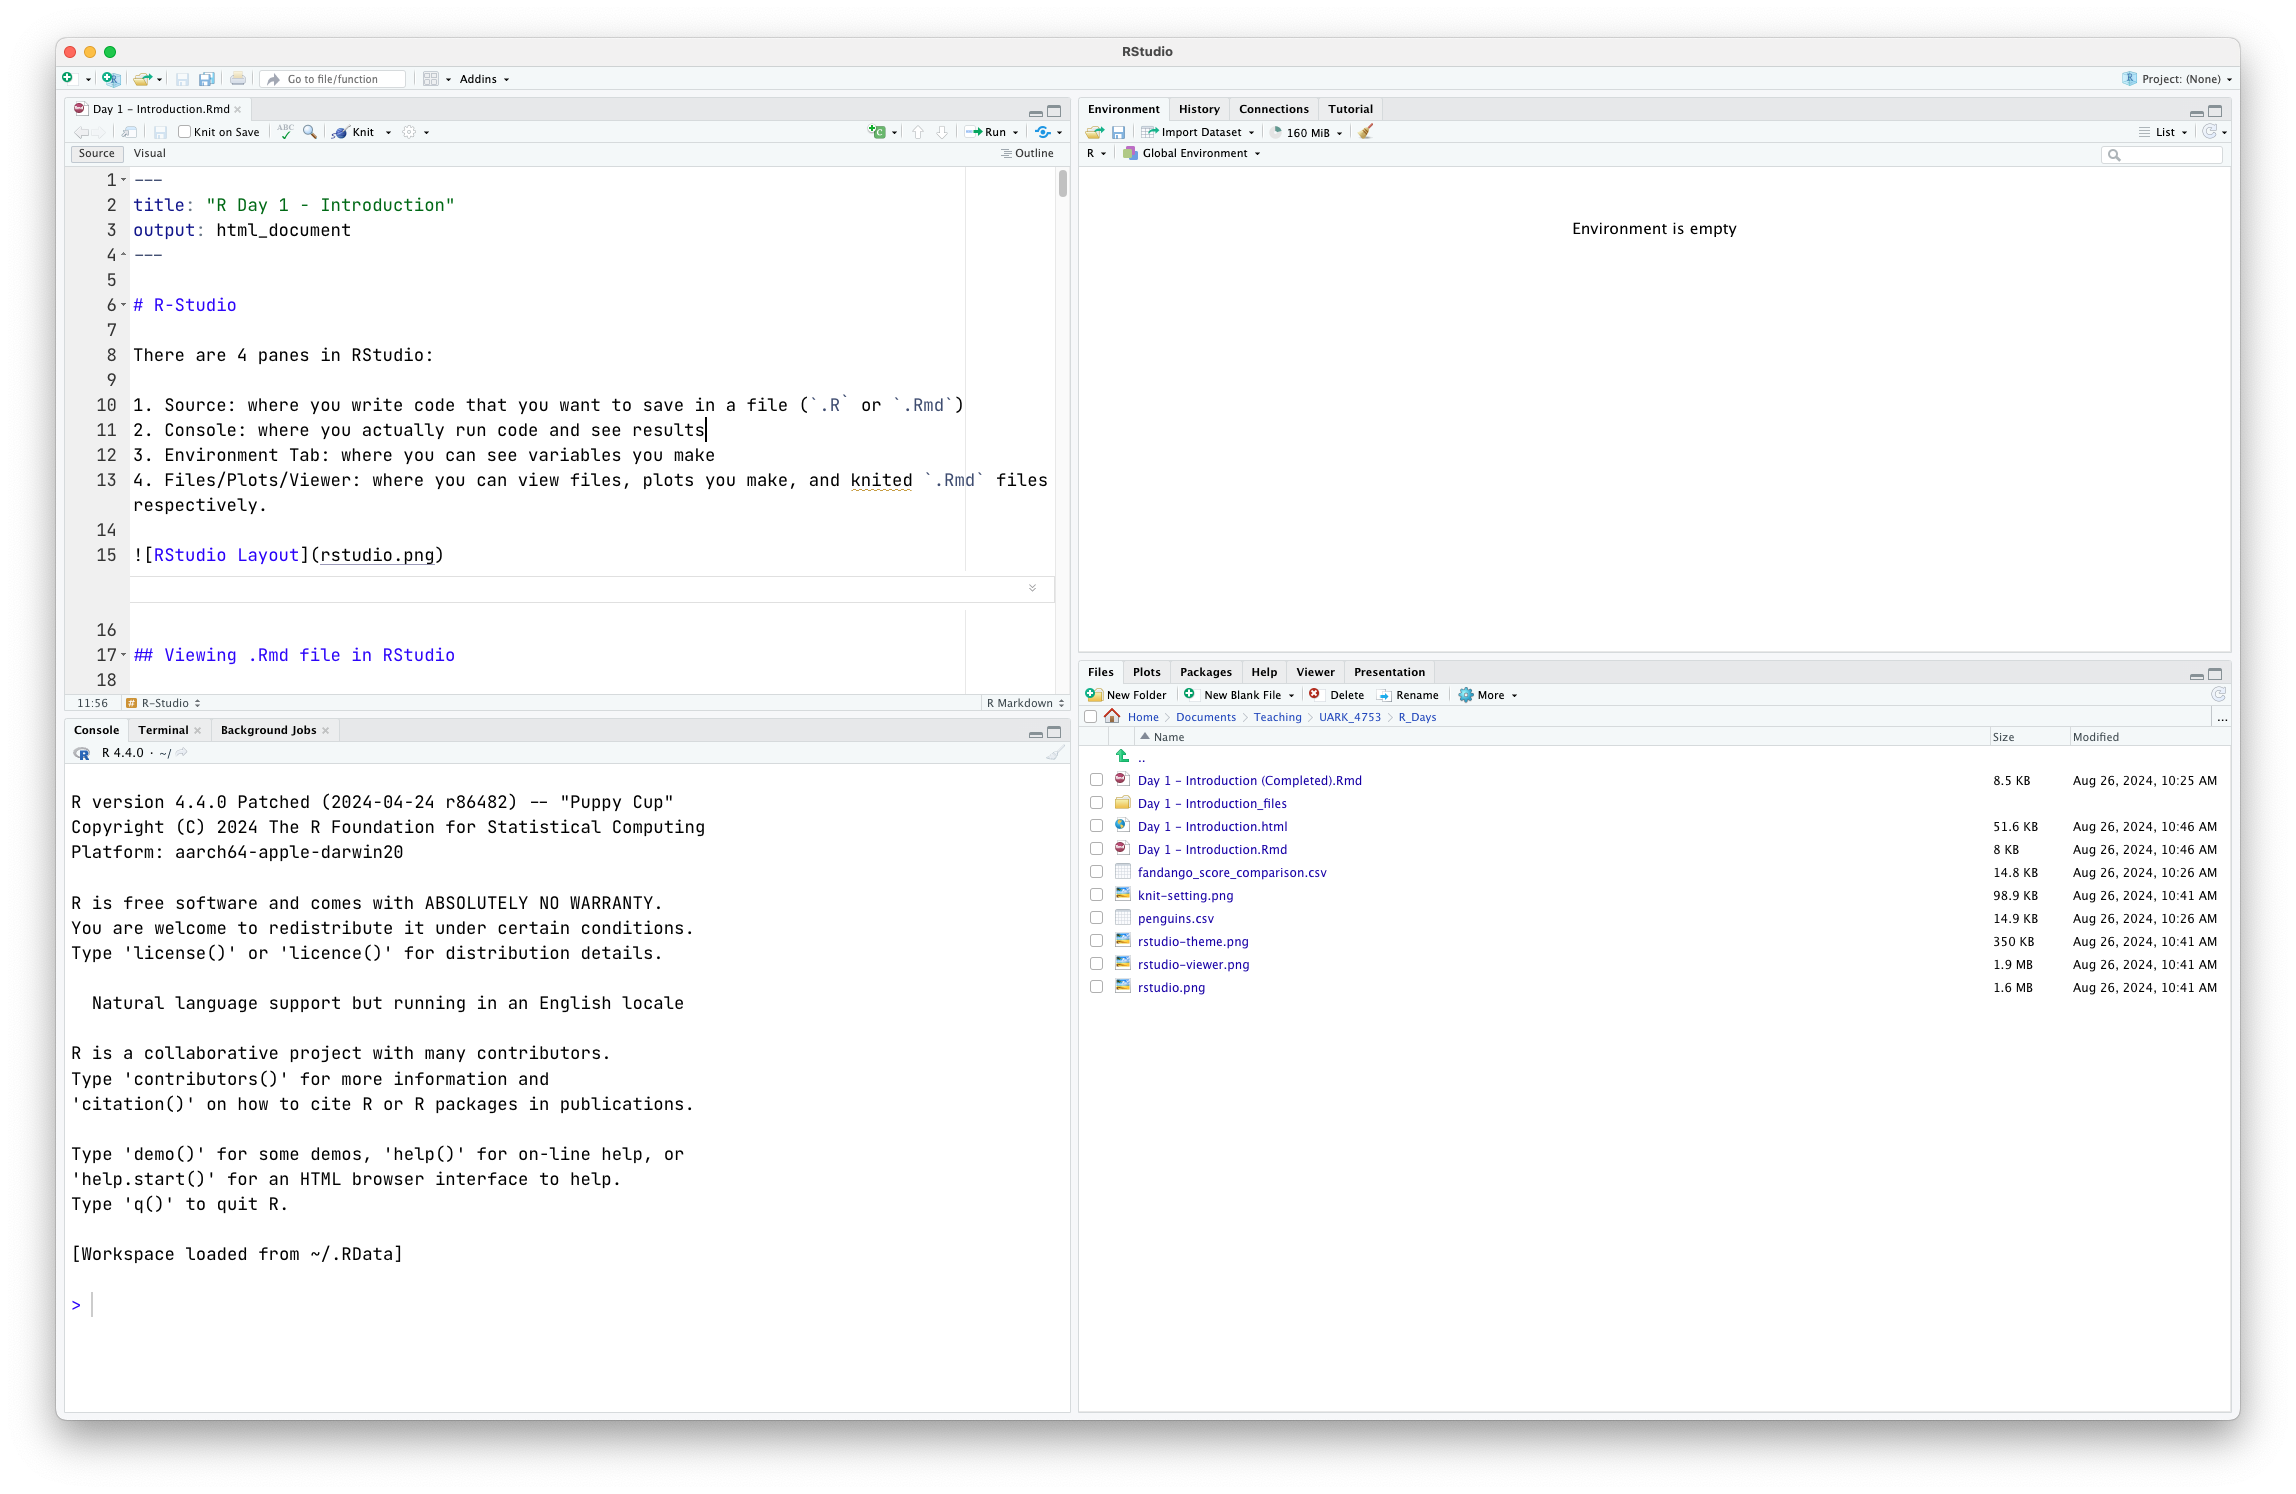
\includegraphics[width = 0.8\textwidth]{figures/rstudio_open_rmd.png}
\end{figure}

\subsection*{Working with RMarkdown files}

For your first homework, you should have completed this interactive tutorial to teach you \href{https://www.markdowntutorial.com/}{markdown syntax} and read this guide on \href{https://evalf21.classes.andrewheiss.com/resource/rmarkdown/}{using RMarkdown}. For that reason, I am going to skip writing out notes on these topics.

When completing assignments, you can run individual blocks as you work to make sure the results come out correctly. You can do this in a few ways. First, you could copy the text from the RMarkdown code chunk (not including the \`{}\`{}\`{} parts) and paste into the console. This is the least effective method but works. Alterantively, you could hit the little green arrow on the right-hand side of the code chunk in RStudio. This will run the code and display the results below the code chunk. 

The third option is for experts. Instead of using your mouse and clicking the button, you could instead use the keyboard shortcut \texttt{Cmd + Enter} on Mac or \texttt{Ctrl + Enter} on Windows. This will run whatever code cell the cursor currently is within.

\begin{tcolorbox}[boxrule = 0pt, frame hidden, sharp corners, enhanced, borderline west = {4pt}{0pt}{kings_river}, interior hidden]
  {\large \textbf{Important:}}

  \smallskip
  You should be careful to include all the code in the RMarkdown file. The reason is that when you go to \textbf{Knit} the RMarkdown file, it is creating a \emph{completely new R instance} and running the code from the top of the RMarkdown file to the bottom. So you should be careful to not use variables that are not defined \emph{above} the cell.
  
  The most common problem students face is loading a csv in the console or through RStudio's interactive data loader and then not including that in the RMarkdown file. 
\end{tcolorbox}

Above your Rmarkdown file, you can see a little ball of yark and the word \textbf{Knit}. This is how you render your Rmarkdown file to an output report. As a default, the knitted document will open up in a separate tab. I do not really like this and you can change this option to view in the \textbf{Viewer} tab. To do so, click the gear and select "Preview in Viewer Pane".

\begin{figure}[!ht]
  \caption{Knit Setting}
  \label{fig:rstudio_knit_setting}
  \centering
  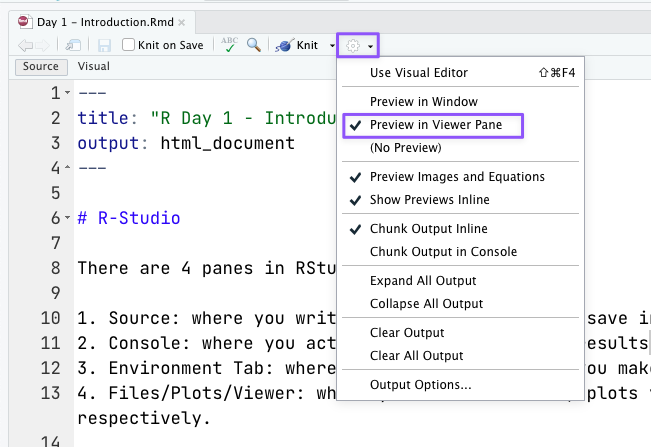
\includegraphics[width = 0.8\textwidth]{figures/rstudio_knit_setting.png}
\end{figure}



\subsection*{RStudio Theme}

If you have a career where you use code (I think quite likely), then you will spend a lot of time in your \textbf{code IDE} (interactive development environment). For that reason, I encourage you to personalize it. 
You can open up RStudio settings and select a theme you enjoy. 
To do so, go in Appearance and click through Editor Themes. 

\begin{figure}[!ht]
  \caption{Theme Selection}
  \label{fig:rstudio_theme}
  \centering
  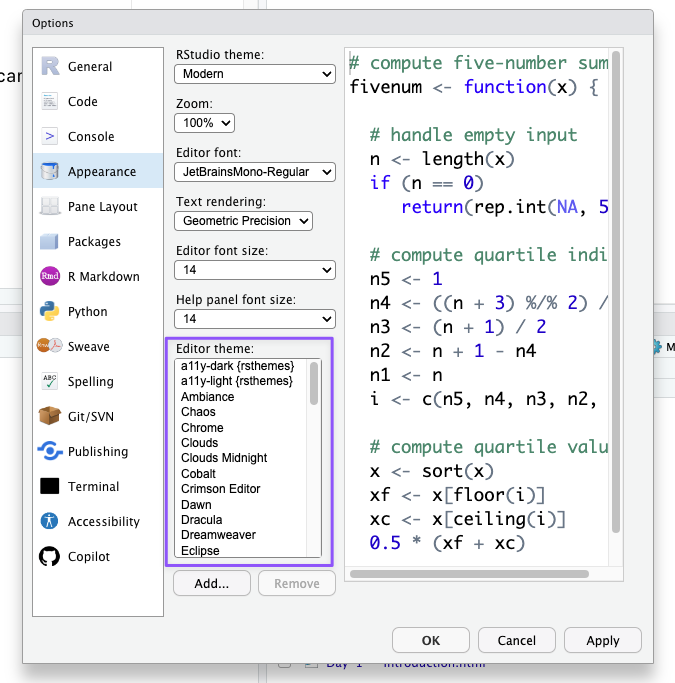
\includegraphics[width = 0.5\textwidth]{figures/rstudio_theme.png}
\end{figure}

Second, you will want a font that is nice to look at. 
You should use a monospace font because it is essential for coding. 
I recommend one of the following:
\begin{itemize}
  \item \href{https://www.jetbrains.com/lp/mono/}{JetBrains Mono},
  \item \href{https://github.com/tonsky/FiraCode}{FiraCode}, or
  \item \href{https://monaspace.githubnext.com}{Monaspace}
\end{itemize}















\end{document}
